\documentclass[a4paper,draft,titlepage]{report} 
% twoside per rilegatura
% twoside: fronte/retro;
% titlepage: pagina del titolo isolata; 
% draft: visualizza righe scritte in modo non ottimale, non mostra le immagini;
% openany: inizia i capitoli in nuove pagine
% \part e \chapter non si possono usare in article, \part non cambia la numerazione dei \chapter

 
%------------------------------------------ Definizione pacchetti ----------------------------------------------%
\usepackage[T1]{fontenc}     % codifica dei font
\usepackage[utf8]{inputenc}  % lettere accentate da tastiera
\usepackage[italian]{babel}  % lingua del documento, l'ultima nelle quadre è la principale
\usepackage{url}             % per scrivere gli indirizzi di internet
\usepackage[final]{graphicx} % final mi mostra anche le immagini nella prewiewhttps://www.overleaf.com/project/5ed402f854c75a0001d3eda8
\usepackage{upgreek}         % lettere greche
\usepackage{amsmath}         % per ad esempio multline
\usepackage{mathtools}
\usepackage{geometry}
\usepackage{listings}
\usepackage{subfig}
\usepackage{caption}
\usepackage{booktabs}
\usepackage{verbatim}
\usepackage{listings}
\usepackage{setspace}
\usepackage{newlfont}
\usepackage{version}
\usepackage{multirow}
\usepackage{gensymb}

\usepackage[section]{placeins} %https://tex.stackexchange.com/questions/279/how-do-i-ensure-that-figures-appear-in-the-section-theyre-associated-with

% https://tex.stackexchange.com/questions/118662/use-placeins-for-subsections
\makeatletter 
\AtBeginDocument{%
  \expandafter\renewcommand\expandafter\subsection\expandafter{%
    \expandafter\@fb@secFB\subsection
  }%
}
\makeatother
\linespread{1.2}


\begin{document}
	
\begin{titlepage}
\begin{center}
{{\LARGE{\textsc{Universit\`a  di Pisa}}}} 
\rule[0.1cm]{14.7cm}{0.1mm}
\rule[0.8cm]{14.7cm}{0.6mm}
{\large{\bf
Corso di Laurea in Ingegneria Robotica \\e dell'Automazione}}
\end{center}
\vspace{5mm}
 \begin{figure}[h]
	\centering
	
\includegraphics[width=0.3\textwidth]{Immagini/unipi}	
\end{figure}

\begin{center}
{\LARGE{\bf \baselineskip=32pt{Progetto di Sistemi di Guida e Navigazione}}}\\
\vspace{20mm} {\Large{\bf Utilizzo di un drone Crazyflie per l'inseguimento del moto di una Active-Wand avvalendosi del sistema di visione Vicon}}
\end{center}
\vspace{10mm}
\par
\noindent
\begin{center}{\textwidth}
\vspace{12mm}
{\large{\bf \vspace{-5pt}Studenti:\\ }}
\end{center}

\begin{center}
{\large{\vspace{-5pt}Alessio Fornaciari, Giacomo Fanfani\\}}
\end{center}
\vspace{30mm}
\rule[0.1cm]{14.1cm}{0.1mm}

\hfill

\vspace{30mm}

\end{titlepage}

	\tableofcontents
\thispagestyle{empty}
\newpage

% Parte 1----------------------------------------------------------------------
\setcounter{page}{1}

\chapter*{Presentazione Hardware}
\addcontentsline{toc}{chapter}{Presentazione Hardware}
\section*{Introduzione}
\addcontentsline{toc}{section}{Introduzione}

Questa relazione è stata da noi pensata non solo come strumento di sintesi di quanto da noi fatto in merito a questo progetto ma anche come possibile "manuale" per chi dopo di noi vorrà continuare il lavoro svolto fino ad ora. Pertanto per iniziare forniremo una breve descrizione dell’hardware da noi utilizzato durante tutto il progetto. 

\section*{Drone Crazyflie}
\addcontentsline{toc}{section}{Drone Crazyflie}

\begin{figure}[h]
    \centering
    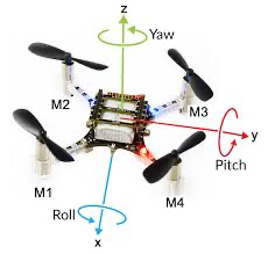
\includegraphics[width=0.6 \textwidth]{Relazione/Immagini/Crazyflie_assi.png}	
    \caption{Drone e relativo sistema di riferimento Body}
    \label{fig:Crazyflie_assi}
\end{figure}

Il nostro drone è un Crazyflie prodotto da BitCraze del tutto equivalente a quello mostrato sopra con l'aggiunta del fatto che sul nostro abbiamo montato anche una piattaforma nella parte superiore che permettesse il posizionamento dei marker, indispensabili per permettere l’individuazione del Drone da parte delle telecamere, e che mostreremo di seguito. 

\section*{Markers}
\addcontentsline{toc}{section}{Markers}

\begin{figure}[h]
    \centering
    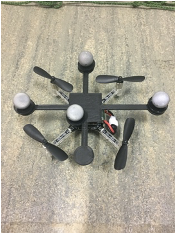
\includegraphics[width=0.6 \textwidth]{Relazione/Immagini/Markers.png}	
    \caption{Piattaforma per posizionamento Markers}
    \label{fig:Markers}
\end{figure}

Al fine di permettere la corretta individuazione del Drone da parte delle telecamere, abbiamo sviluppato un’apposita piattaforma che è stata poi stampata e apposta sulla parte superiore al fine di permettere un migliore posizionamento dei marker. Dato che marker troppo vicini davano fastidio al sistema di visione, abbiamo scelto una piattaforma che si estendesse maggiormente in ampiezza rispetto a quella originale grazie ai prolungamenti che riescono a passare tra le eliche senza dare loro fastidio durante il volo. Il colore nero è preferibile in quanto tra tutti è quello che meno riflette e che causa quindi minori interferenze con le telecamere. La disposizione dei maker è arbitraria purchè siano fissati in modo rigido e non crei una geometria simmetrica, ciò è necessario in quanto durante il movimento del Drone il sistema di visione deve poter riconoscere l’orientamento del Drone senza ambiguità, non si devono dunque verificare casi in cui la disposizione dei marker potrebbe corrispondere a due o più diverse configurazioni del Drone, in quel caso infatti il sistema non riuscirebbe a riconoscere l'orientazione corretta del Drone e fornirebbe quindi valori di orientazione errati rispetto a quelli reali. 

\section*{Eliche}
\addcontentsline{toc}{section}{Eliche}

\begin{figure}[h]
    \centering
    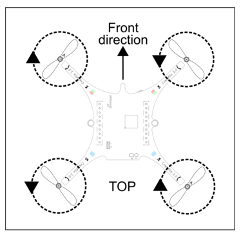
\includegraphics[width=0.6 \textwidth]{Relazione/Immagini/Eliche.png}	
    \caption{Corretto posizionamento delle eliche}
    \label{fig:Eliche}
\end{figure}

Dato che può capitare che un esperimento non vada come previsto e termini con una caduta del Drone, una breve parentesi sul corretto montaggio delle eliche è necessaria in quanto potrebbe succedere che nella caduta alcune si stacchino dal relativo albero. 
Nel caso in qui questo succeda è necessario tenere a mente che le eliche sono di due tipi e che, come indica la figura, il montaggio non è del tutto arbitrario ma deve seguire la seguente logica: 
\begin{itemize}
    \item \verb Eliche  \verb di  \verb tipo  \verb A2:  queste devono essere montate sui motori il cui verso di rotazione è quello orario. 
    \item \verb Eliche  \verb di  \verb tipo  \verb B2:  al contrario, devono essere montate sui motori il cui verso di rotazione è quello  antiorario.
\end{itemize}

Si fa notare che le eliche dello stesso tipo saranno alla fine disposte l’una di fronte all’altra (non accanto) e che il verso di rotazione di ciascun motore è riportato sui terminali del drone come ultimo simbolo. \\ 
Nel momento in cui queste vengono rimontate è bene fare una pressione abbastanza forte in modo da assicurarsi che non si stacchino più con facilità. 

\section*{Crazyradio}
\addcontentsline{toc}{section}{Crazyradio}


\begin{figure}[h]
    \centering
    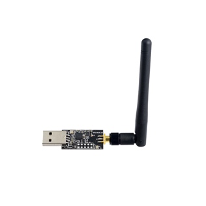
\includegraphics[width=0.4 \textwidth]{Relazione/Immagini/Crazyradio.png}
    \caption{Crazyradio}
    \label{fig:Crazyradio}
\end{figure}
\\
\\
\\
\\
\\
\\
\\
\\
\\
\\
\\
\\
\\
\\
\\
\\


Per poter comunicare il Drone utilizza il protocollo CRTP appositamente sviluppato da Bitcraze (verrà descritto nel dettaglio più avanti). \\ 
La Crazyradio è il mezzo che consente la comunicazione bidirezionale tra il pc su cui essa è installata e il Drone. 

\section*{Vicon Active Wand}
\addcontentsline{toc}{section}{Vicon Active Wand}

\begin{figure}[h]
    \centering
    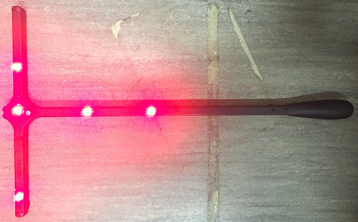
\includegraphics[width=0.5 \textwidth]{Relazione/Immagini/Wand.png}
    \caption{Vicon Active Wand in funzione}
    \label{fig:Wand}
\end{figure}

Questa è la “Bacchetta” da noi utilizzata come target da inseguire. Come si nota ha già installati dei piccoli laser che una volta accesi fungono da marker. A differenza dei marker del drone (passivi) questi sono marker attivi e dunque conenstono un tracciamento molto più preciso da parte delle telecamere. \\
A volte è anche utilizzata per ricalibrare l’intero sistema e fornire posizione e orientazione della terna fissa (da noi rinominata come  "terna Vicon"). La ricalibrazione è consigliata all'inizio di ogni sessione di esperimenti, in alternativa, ogni volta che si verificano cambiamenti in termini di "fantasie" di pavimentazione, luce, temperatura … Diventa praticamente obbligatoria invece nel momento in cui il Software non riesce a visualizzare correttamente i marker (attivi o passivi) posti sugli oggetti, può anche accadere che ne vengano mostrati più di quanti in realtà sono presenti sui relativi oggetti. 

\section*{Vicon Tracker}
\addcontentsline{toc}{section}{Vicon Tracker}

\begin{figure}[h]
    \centering
    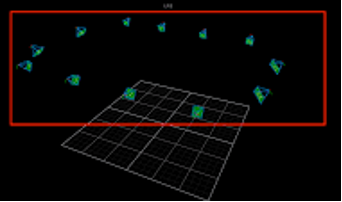
\includegraphics[width=0.6 \textwidth]{Relazione/Immagini/Tracker.png}
    \caption{Software Tracker in funzione con evidenziate in rosso le telecamere disposte nella flight room, il cui pavimento è rappresentato dalla griglia.}
    \label{fig:Tracker}
\end{figure}

Il Sistema di tracciamento Vicon è in realtà costituito sia da Hardware che da Software, più precisamente il Software di Tracking si avvale delle telecamere, posizionate nella flight room, per individuare i Markers posti sugli oggetti. \\
In figura si mostrano le telecamere così come appaiono dal software. \\
Inizialmente (e periodicamente) il sistema ha bisogno di una ricalibrazione grazie alla quale, con l'ausilio della Wand, viene fatto un reset delle impostazioni delle telecamere per renderle pù precise; vengono inoltre reimpostate sia l'origine della terna fissa (solitamente posta al centro della stanza) che l'orientazione dei relativi assi. \\
Una volta calibrato, il sistema deve essere in grado di individuare in modo esatto i markers piazzati sugli oggetti. Questi possono essere selezionati in gruppo per creare degli "oggetti software" da associare ai "dispositivi fisici". Tra le proprietà (campi) più utili di questi oggetti troviamo il nome, utilizzato come "alias" all'interno del codice Python, e i sistemi di riferimento "body", che devono essere opportunamente inzializzati con posizione e orientazione desiderati (in alternativa il sistema li inizializza nel modo che sul momento ritiene più adatto, è dunque sempre consigliato di reimpostarli manualmente). 
\chapter*{Panoramica generale del Progetto}
\addcontentsline{toc}{chapter}{Panoramica generale del Progetto}

Scopo del progetto è quello di integrare tutti i dispositivi precedentemente descritti al fine di realizzare l’inseguimento, da parte del Drone, del moto della Wand all’interno della flight-room avvalendosi del sistema di posizionamento Vicon che fornisce sia la misura di “posizione target” della Wand che la misura di posizione del Drone, quest’ultima da utilizzare in ingresso al filtro di Kalman del Drone stesso per l'aggiornamento della sua posizione corrente. \\
In realtà il sistema Vicon fornisce anche misure di orientazione (fornite tramite relativi quaternioni) che però per quanto riguarda la Wand non sono di interesse per gli scopi di questo progetto mentre, per quanto riguarda il drone, sono stati oggetto di molte sperimentazioni che purtroppo ad oggi non hanno ancora consentito di utilizzarli in modo "completo", in particolare il progetto allo stato attuale utilizza le misure di orientazione del Drone soltanto per effettuare delle conversioni tra i sisitemi di riferimento utilizzati, non prende invece in considerazione tali misure come ingressi al filtro di Kalman del Drone. \\
\\
Di seguito presentiamo uno schema concettuale con le connessioni stabilite tra i vari componenti, accompagnato da una breve descrizione:
\begin{figure}[h]
    \centering
    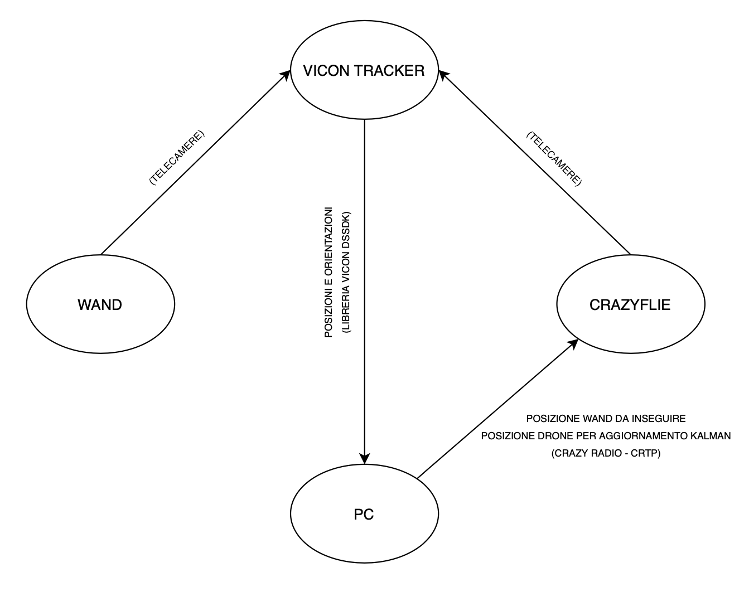
\includegraphics[width=0.8 \textwidth]{Relazione/Immagini/Generale_Progetto.png}
    \caption{Schema a blocchi delle entità coinvolte nel progetto}
    \label{fig:Generale_Progetto}
\end{figure}
\\
\begin{itemize}
    \item Le telecamere, tramite l’individuazione dei marker posizionati sugli oggetti, permettono al Tracker di ricavare in ogni istante posizioni e orientazioni di Drone e Wand;
    \item Tramite le funzioni della libreria Vicon-DSSDK il programma in esecuzione riceve dal tracker le posizioni e le orientazioni di interesse;
    \item Il programma elabora posizioni e orientazioni effettuando eventuali conversioni tra sistemi di riferimento e tramite la Crazyradio e le librerie Python che implementano il protocollo CRTP:
    \begin{itemize}
        \item Fornisce al Drone i nuovi riferimenti di posizione da inseguire, ricavati dalla posizione aggiornata della Wand;
        \item Fornisce al Drone le nuove misure della sua posizione da utilizzare per l’aggiornamento del filtro di Kalman.
    \end{itemize}
    \item E cosi via .. 
\end{itemize}
\\
(più avanti dedicheremo un paragrafo per scendere nel dettaglio di tutte le operazioni necessarie)

\chapter*{Breve Panoramica sul Protocollo CRTP}
\addcontentsline{toc}{chapter}{Breve Panoramica sul Protocollo CRTP}

Il protocollo CRTP (Crazy Real Time Protocol) è il protocollo creato appositamente da Bitcraze per gestire la comunicazione da/verso il Drone. 
\\
Concettualmente la comunicazione che avviene tra il Drone e la Crazyradio segue il seguente schema: 
\begin{figure}[h]
    \centering
    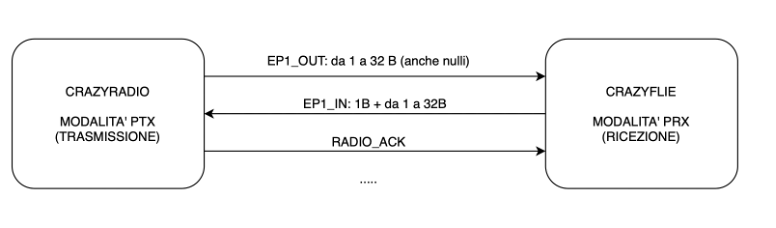
\includegraphics[width=0.8 \textwidth]{Relazione/Immagini/handshake.png}
    \caption{Handshake CRTP}
    \label{fig:Handshake}
\end{figure}
\\
Le relative implementazioni Python dei due blocchi sopra mostrati sono le seguenti: 

\begin{figure}[h]
    \centering
    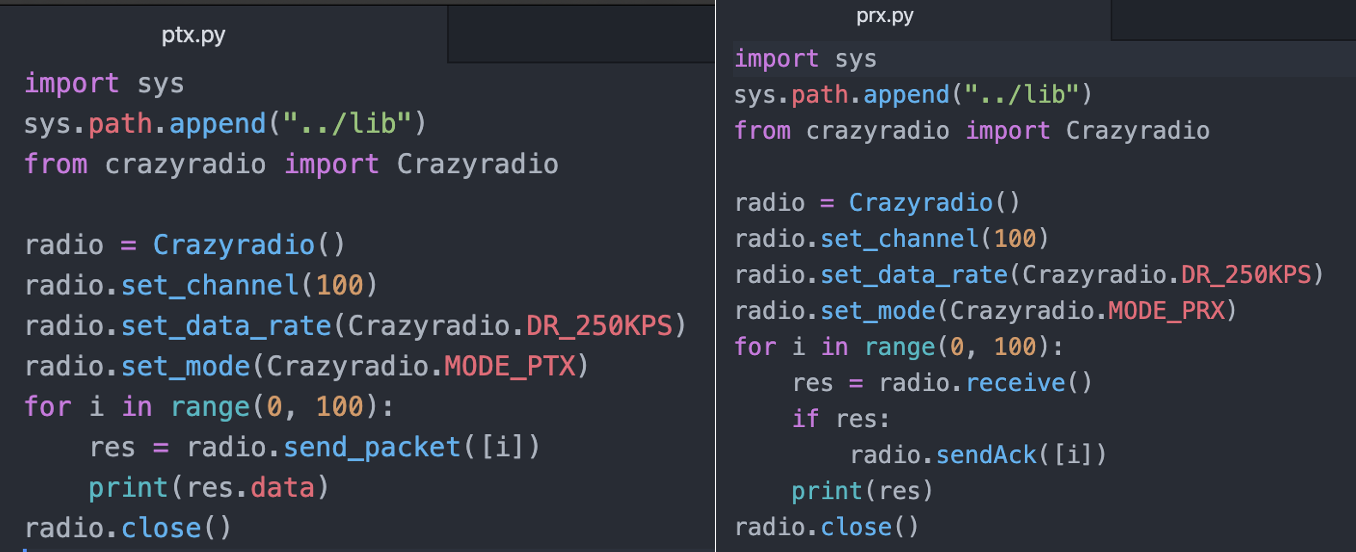
\includegraphics[width=0.8 \textwidth]{Relazione/Immagini/HandshakePython.png}
    \caption{Handshake CRTP con funzioni Python}
    \label{fig:HandshakePyhton}
\end{figure}
\\
Andando più nel dettaglio abbiamo visto come questo protocollo  si avvale di  pacchetti che hanno la seguente struttura: 
\\
\begin{figure}[h]
    \centering
    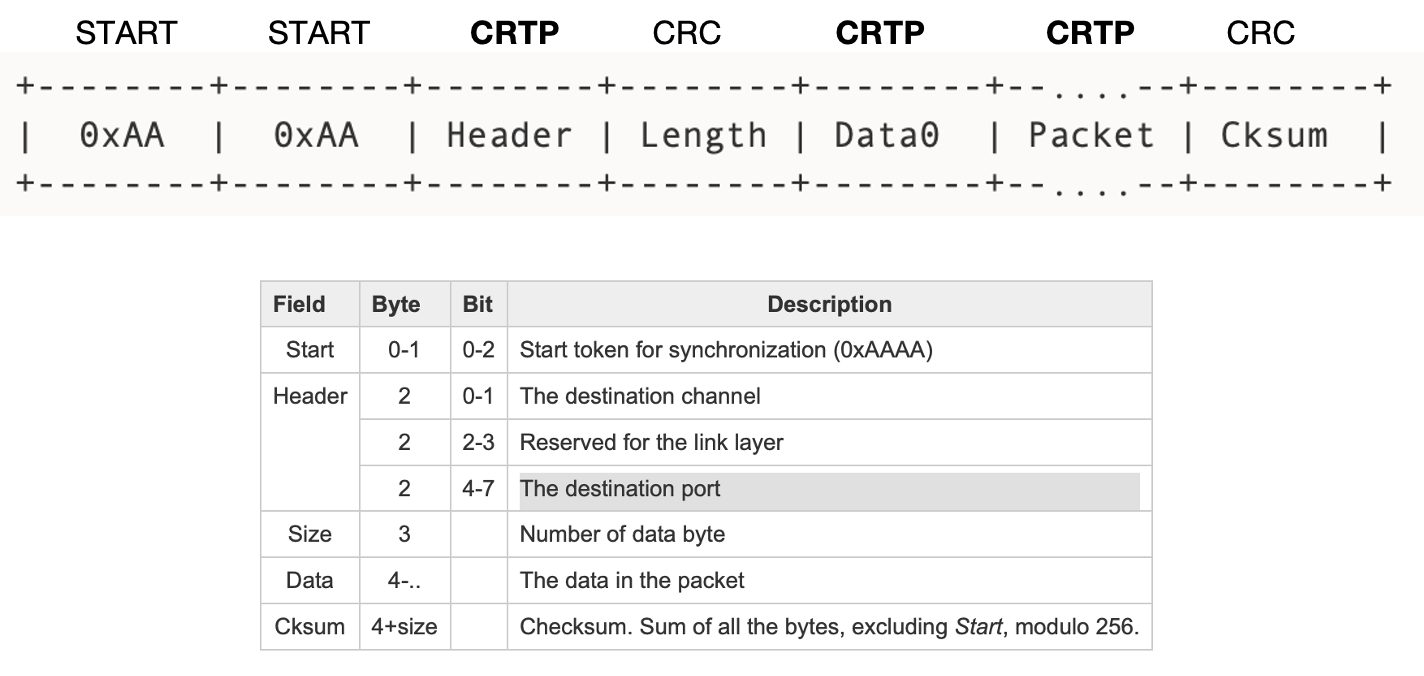
\includegraphics[width=0.8 \textwidth]{Relazione/Immagini/PacchettiCRTP.png}
    \caption{Pacchetti CRTP - Specifichiamo che il campo Data può contenere al massimo 31B}
    \label{fig:PacchettiCRTP}
\end{figure}
\\
Un’ulteriore analisi della codifica della Porta di destinazione è necessaria: \begin{figure}[h]
    \centering
    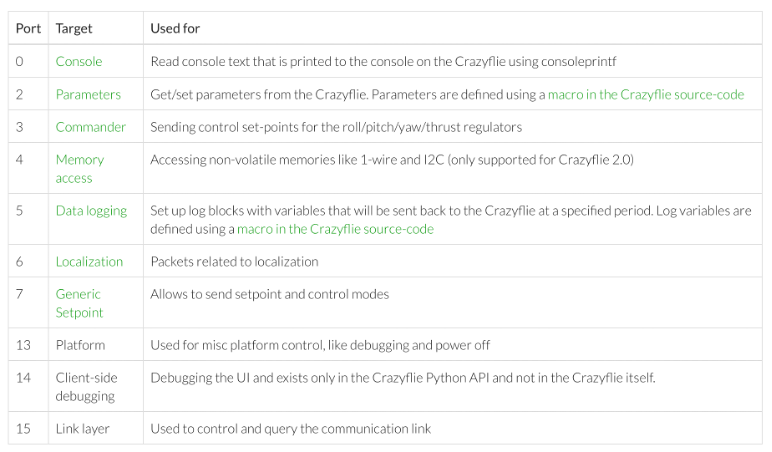
\includegraphics[width=0.8 \textwidth]{Relazione/Immagini/PorteDestinazione.png}
    \caption{Codifica porte di destinazione dei pacchetti CRTP}
    \label{fig:PorteDestinazione}
\end{figure}
\\
Di seguito riportiamo un banale esempio in cui vediamo come dovrebbe essere fatto un pacchetto per voler inviare al \verb Commander  (porta 3) un campo \verb Data  contenente riferimenti nulli di orientazione e spinta dei motori:
\begin{figure}[h]
    \centering
    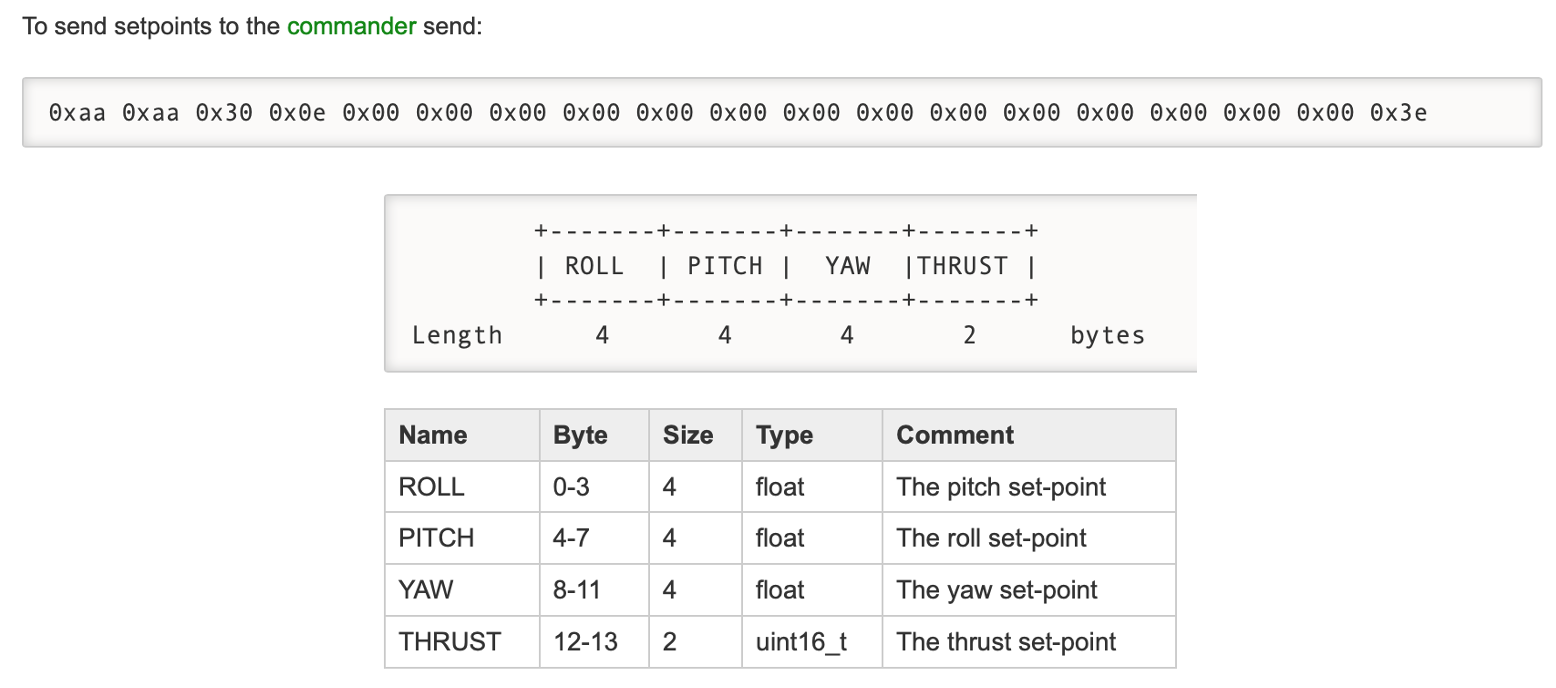
\includegraphics[width=0.9 \textwidth]{Relazione/Immagini/EsempioCommander.png}
    \caption{Esempio di invio pacchetto CRTP}
    \label{fig:EsempioCommander}
\end{figure}
\\
\\
\\
\\
\\
\\
\\
Tornando  allo scopo del progetto, è per noi di interesse la porta 6 utilizzata per la trasmissione di pacchetti contenenti informazioni di posizione e orientazione.  \\
Di seguito vediamo come, tramite la codifica di due diversi “canali”, possiamo utilizzare questa porta per la trasmissione di informazioni automaticamente indirizzate al filtro di Kalman (utilzzando il \textbf{canale 0}):
\begin{figure}[h]
    \centering
    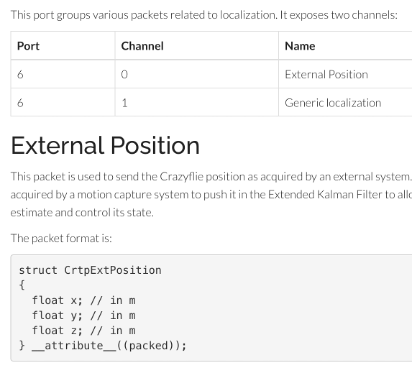
\includegraphics[width=0.6 \textwidth]{Relazione/Immagini/externalposition.png}
    \caption{External Position}
    \label{fig:externalposition}
\end{figure}
\\
\\


Qualora volessimo trasmettere anche l’informazione dell’orientazione, in aggiunta a quella di posizione, dobbiamo avvalerci del \textbf{canale 1} che consente l’invio di una struttura dati di dimensioni maggiori, come mostrato di seguito: 
\begin{figure}[h]
    \centering
    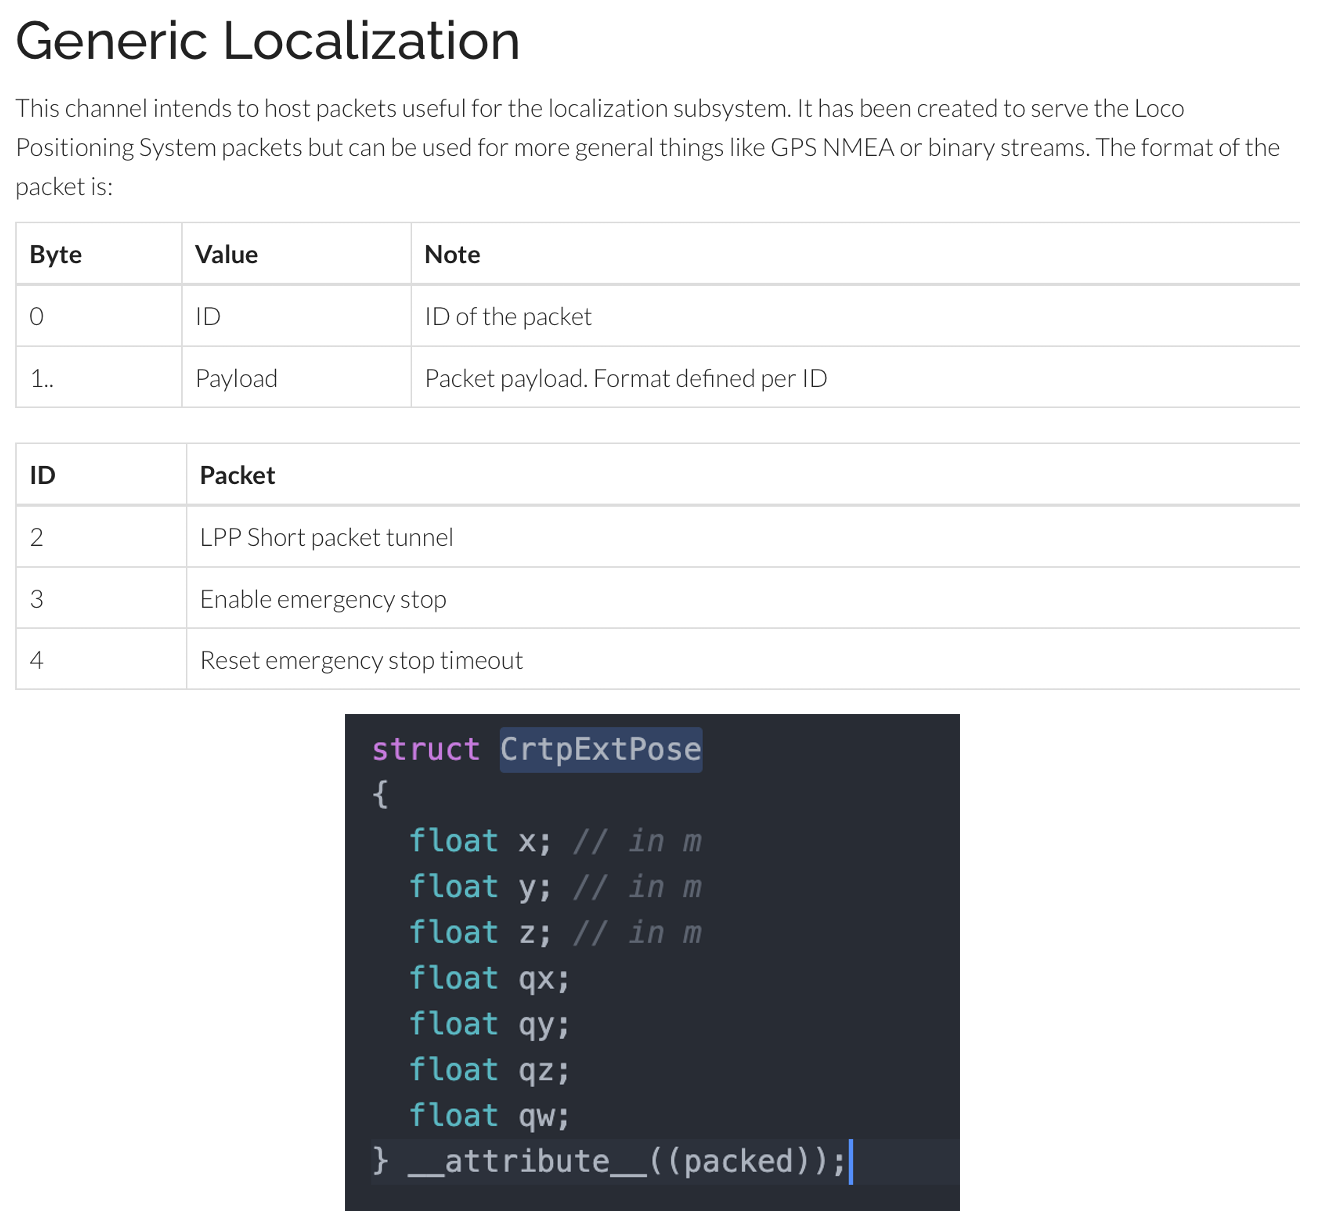
\includegraphics[width=0.8 \textwidth]{Relazione/Immagini/genericLocalization.png}
    \caption{External Position}
    \label{fig:genericLocalization}
\end{figure}


\chapter*{Breve panoramica sulla libreria CFLIB - Python}
\addcontentsline{toc}{chapter}{Breve panoramica sulla libreria CFLIB - Python}
\section*{Riferimenti di Posizione}
\addcontentsline{toc}{section}{Riferimenti di Posizione}

Questa libreria è stata appositamente sviluppata da Bitcraze e contiene tutte le funzioni necessarie per comunicare da/verso il Drone. Essendo open-source al suo sviluppo può contribuire chiunque e c’è molta disponibilità di materiale sul web. 
\\
La libreria contiene svariate classi grazie a cui si possono inviare comandi al Drone, di seguito a titolo di esempio e soltanto per fornire un’idea di come queste funzioni sono implementate, mostreremo alcune delle funzioni e andremo ad analizzarle passando dal vedere come queste sono disponibili “ad alto livello” e guardando come si implementano “a basso livello” fino alle funzioni che implementano l’invio dei pacchetti CRTP spiegati in precedenza. 
\\
Un esempio è la classe \verb Commander  che consente di inviare al Drone riferimenti di posizione da inseguire e che è la stessa utilizzata nel nostro codice. Ne vediamo un estratto in figura ~\ref{fig:funzioniAltoLivello}.
\\
In realtà per essere più precisi specifichiamo che nel codice utilizzeremo anche una variante della classe \verb Commander  e che si chiama \verb MotionCommander  . La particolarità di quest'ultima è che consente di effettuare la procedura di decollo in modo "automatico" una volta creato il relativo oggetto Dorne. Avremo dunque nel nostro codice un oggetto per ognuna di queste due classi ma utilizzeremo questa variante soltanto per effettuare il decollo mentre per l'intera parte rimanente ci avvaleremo della classe \verb Commander . 
\begin{figure}[h]
    \centering
    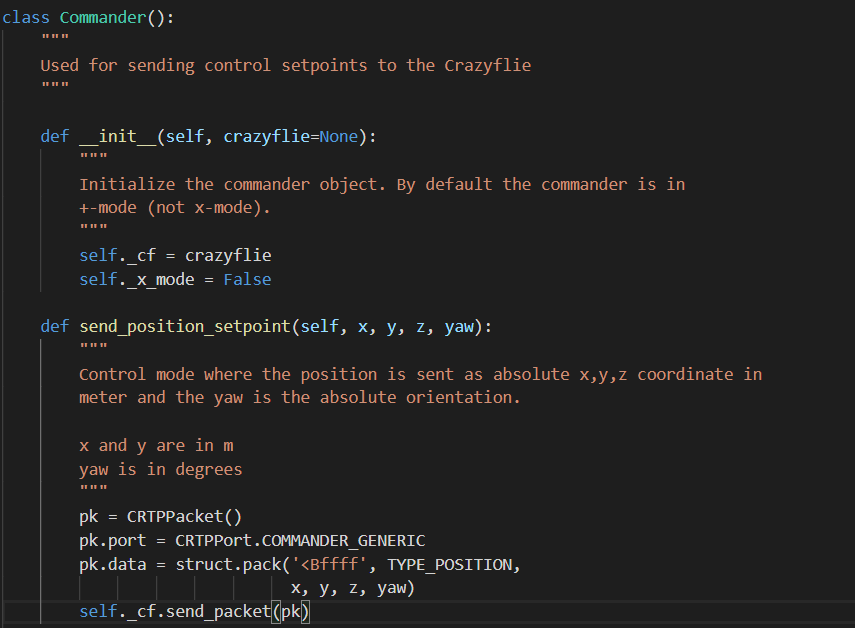
\includegraphics[width=0.8 \textwidth]{Relazione/Immagini/funzioniAltoLivello.PNG}
    \caption{Classe Commander}
    \label{fig:funzioniAltoLivello}
\end{figure}

\\
Al loro interno queste funzioni consentono di costruire i pacchetti CRTP a partire dai valori dei riferimenti desiderati.
L'invio del pacchetto è fatto in accordo con quanto previsto dal protocllo CRTP utilizzando la send\_packet riportata in figura ~\ref{fig:sendPacketPyton}. 
\\
\begin{figure}[h]
    \centering
    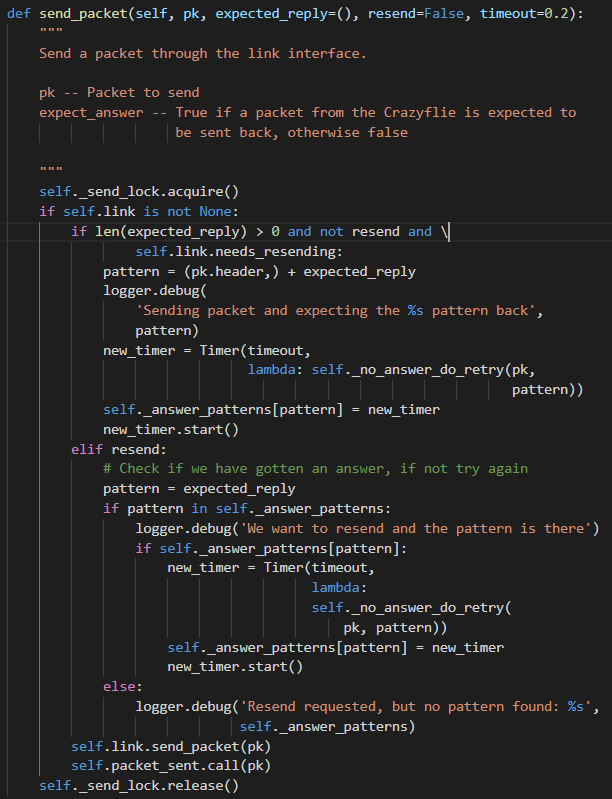
\includegraphics[width=0.8 \textwidth]{Relazione/Immagini/sendPacketPyton.png}
    \caption{send\_packet - Chiamata all'interno della send\_setpoint responsabile del solo handshake iniziale}
    \label{fig:sendPacketPyton}
\end{figure}
\\
A sua volta questa funzione ricorre alle funzioni proprie del driver della Crazyradio. In figura ~\ref{fig:sendPacket} riportiamo la send\_packet che di fatto consente alla Crazyradio di inviare il pacchetto CRTP (notiamo come questa, essendo parte del firmware è scritta in C). 
\\
\begin{figure}[h]
    \centering
    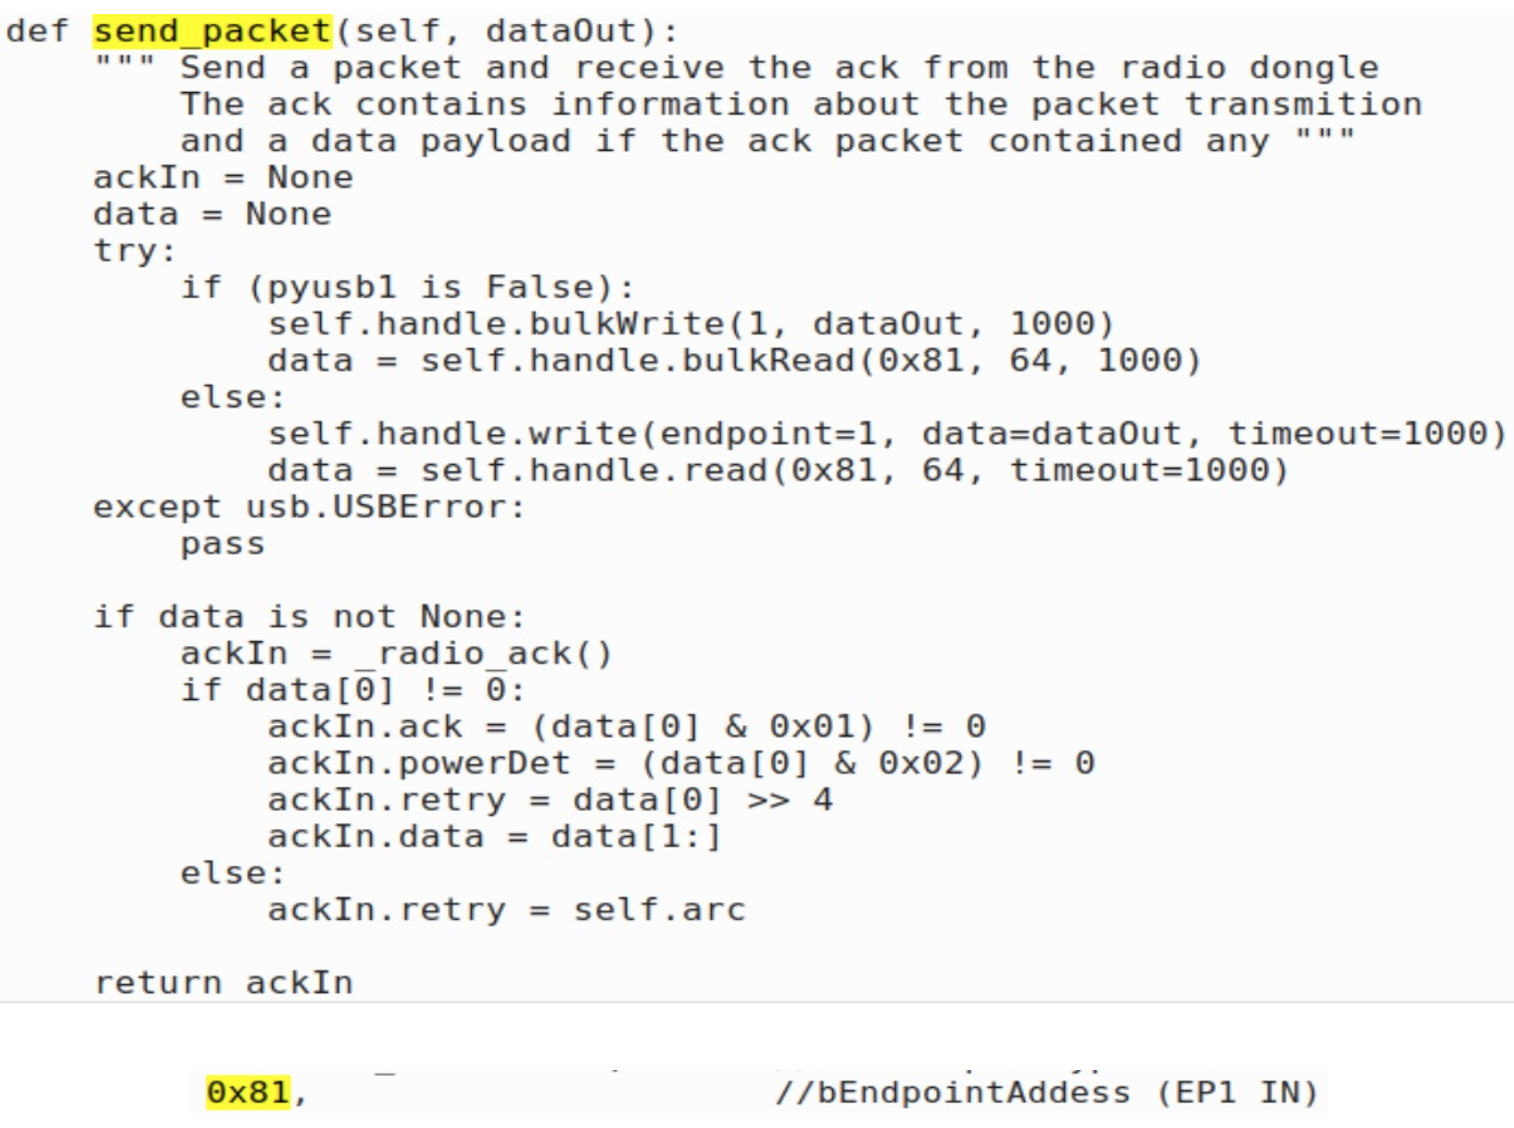
\includegraphics[width=0.8 \textwidth]{Relazione/Immagini/sendPacket.png}
    \caption{send\_packet - Tramite la bulkWrite invia dataOut per poi attendere quanto ricevuto dal Drone e metterlo in data}
    \label{fig:sendPacket}
\end{figure}
\\
\section*{Aggiornamento filtro di Kalman}
\addcontentsline{toc}{section}{Aggiornamento filtro di Kalman}
\\
Per inviare le misure di posizione al filtro di Kalman utilizziamo la funzione \verb send_extpos  che riportiamo in figura ~\ref{fig:sendextpos}.

\begin{figure}[h]
    \centering
    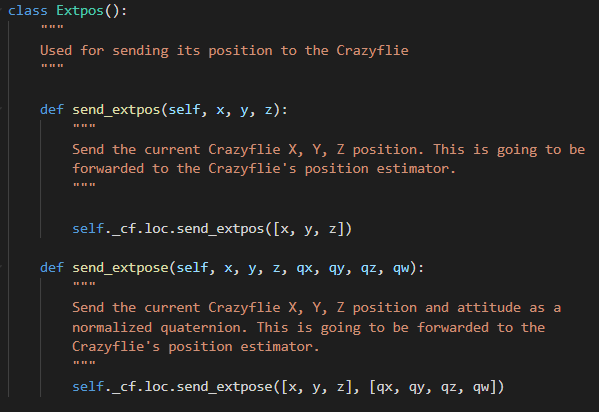
\includegraphics[width=0.8 \textwidth]{Relazione/Immagini/sendextpos.png}
    \caption{In figura sono riportate sia la send\_extpos, utilizzata per l'invio della sola posizione, che la send\_extpose, utilizzata per l'invio di posizione e orientazione}
    \label{fig:sendextpos}
\end{figure}

\\
\\
Per quanto riguarda la gestione dei messaggi nel caso di ricezione (da parte del Drone) di informazioni di posizione da utilizzare per l’aggiornamento del filtro di Kalman, ricordando quanto detto precedentemente, si riporta nelle figure che vanno dalla ~\ref{fig:externalPositionRiassunto} alla ~\ref{fig:genericPositionHandler} il “percorso” (in termini di funzioni della libreria) seguito dal pacchetto una volta ricevuto e “spacchettato” dal Crazyflie.

\begin{figure}[h]
    \centering
    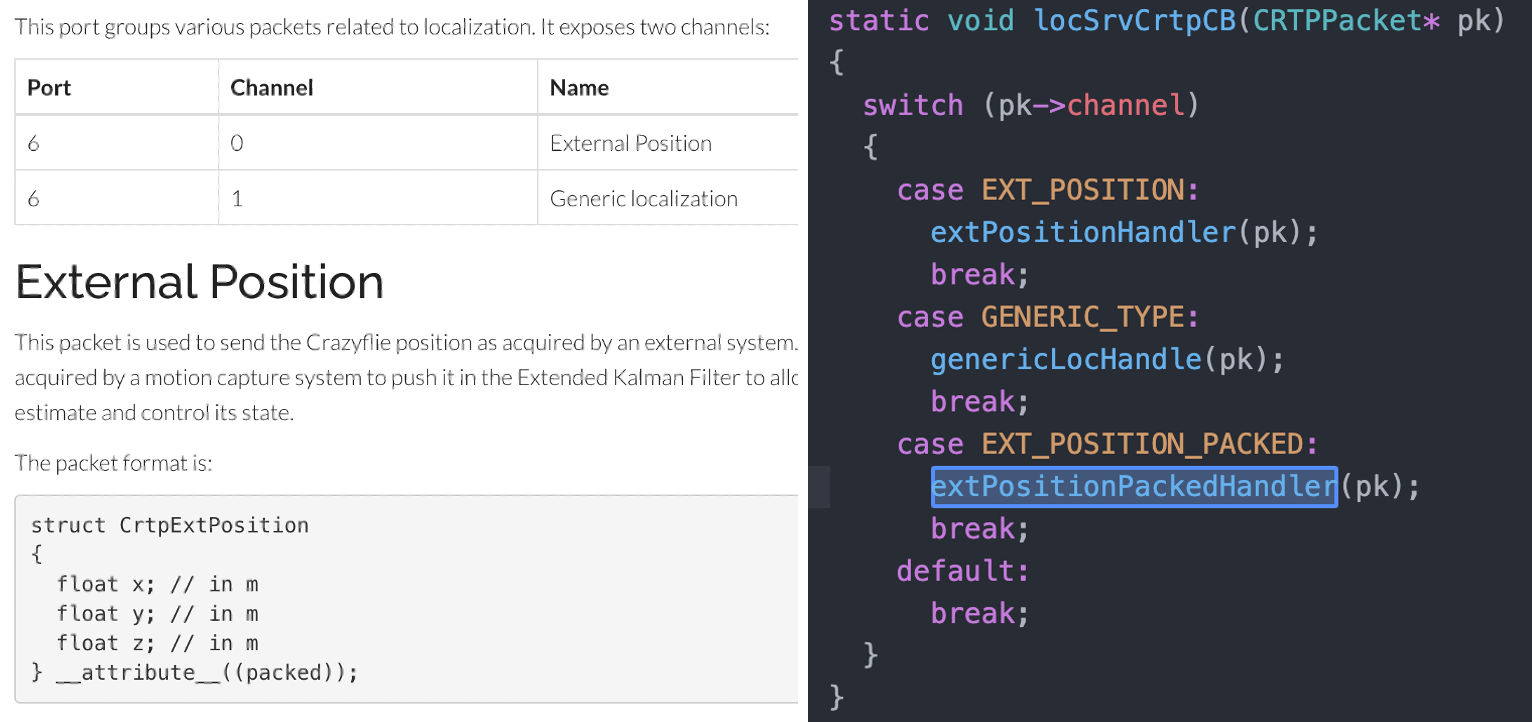
\includegraphics[width=0.8 \textwidth]{Relazione/Immagini/externalPositionRiassunto.png}
    \caption{a seconda del canale scritto nel pacchetto l’informazione viene gestita da funzioni diverse che, a seconda del caso, operano secondo quanto stabilito dal protocollo CRTP}
    \label{fig:externalPositionRiassunto}
\end{figure}
\\
\begin{figure}[h]
    \centering
    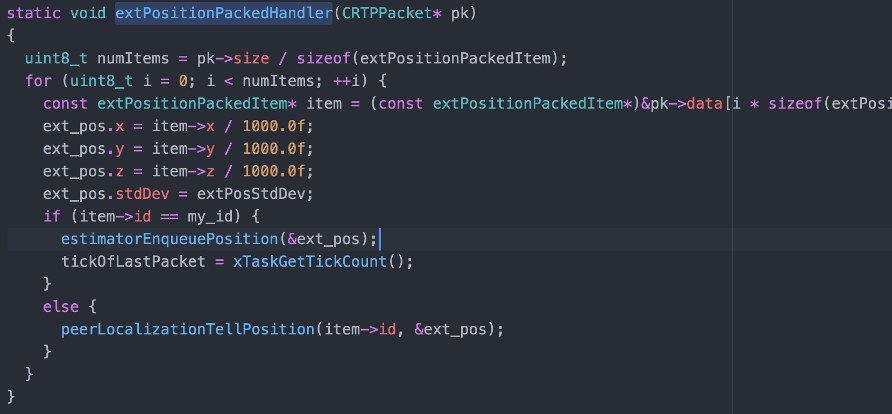
\includegraphics[width=0.8 \textwidth]{Relazione/Immagini/extPositionPackedHandler.png}
    \caption{Qui notiamo l’utilizzo dell’informazione della sola posizione per assegnarla al valore attuale di posizione del Drone e la messa in coda tra i dati da utilizzare per il filtro di Kalman.}
    \label{fig:extPositionPackedHandler}
\end{figure}
\\
\begin{figure}[h]
    \centering
    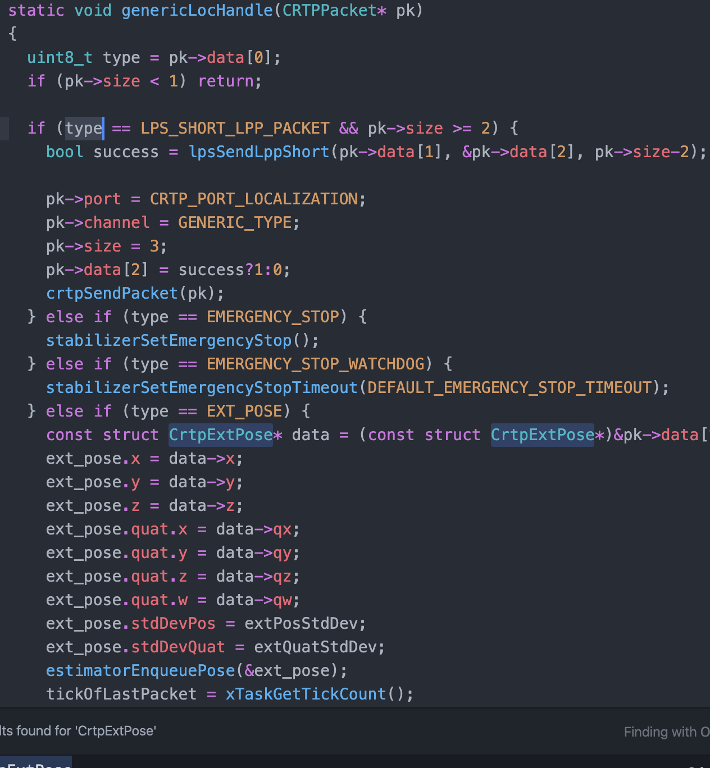
\includegraphics[width=0.8 \textwidth]{Relazione/Immagini/genericPositionHandler.png}
    
    \caption{Qui vediamo invece come viene gestita l’informazione quando riceviamo, oltre alla posizione, anche l’orientazione. 
Il ramo di codice di interesse è quello relativo a “type == EXT\_POSE” (in cui EXT\_POSE vale 8).
}
    \label{fig:genericPositionHandler}
\end{figure}
\\
In entrambi i casi, sia che si passi dalla \verb genericPositionHandler  sia che si passi  dalla \\ \verb extPositionHandler 
, una volta inseriti nella coda i dati vengono elaborati come in figura ~\ref{fig:kalmanCoreUpdate}. 
\\
\begin{figure}[h]
    \centering
    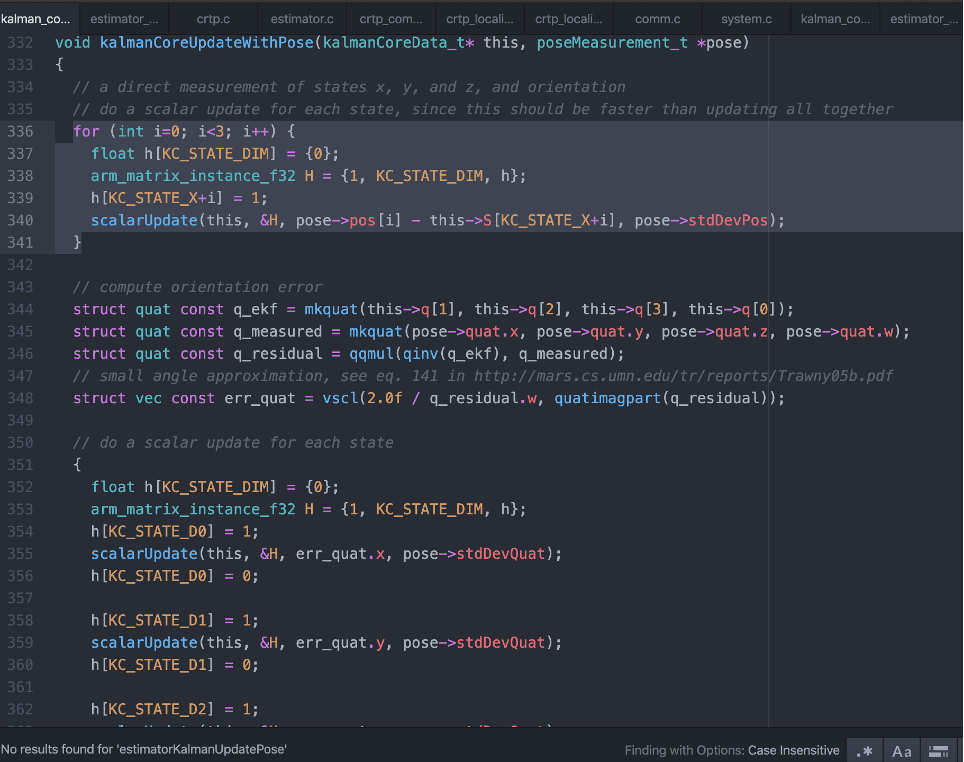
\includegraphics[width=0.8 \textwidth]{Relazione/Immagini/kalmanCoreUpdate.png}
    \caption{}
    \label{fig:kalmanCoreUpdate}
\end{figure}

\chapter*{Breve panoramica sulla libreria Py-Vicon}
\addcontentsline{toc}{chapter}{Breve panoramica sulla libreria Py-Vicon}

Questa libreria è quella che utilizziamo per ottenere dal Tracker le informazioni di posizione e orientazione di Drone e Wand. 
\\
Le uniche funzioni per noi di interesse sono quelle riportate nelle figure ~\ref{fig:getSegmentGlobalRotation} e ~\ref{fig:getSegmentGlobalTranslation}. 
\\
In realtà utilizzeremo anche una terza funzione che ci consente di recuperare l'informazione di orientazione di un oggetto tramite i relativi quaternioni. Questa funzione non è stata riportata in quanto come detto in precedenza il progetto allo stato attuale non "integra" alla perfezione l'utilizzo di questa funzione che sarebbe dovuta servire per aggiornare l'informazione di orientazione del drone nel suo filtro di Kalman. 
\\
\begin{figure}[h]
    \centering
    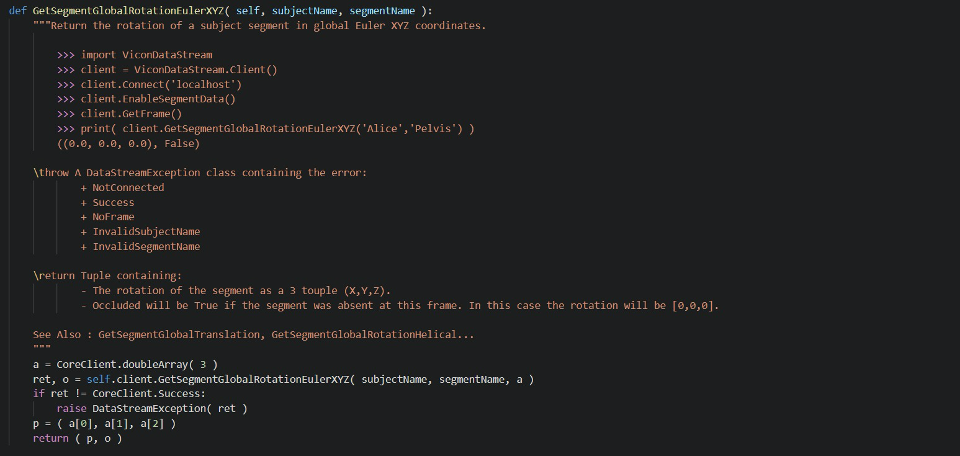
\includegraphics[width=1 \textwidth]{Relazione/Immagini/getSegmentGlobalRotation.png}	
    \caption{Funzione utilizzata per ricevere dal Tracker la matrice di rotazione che rappresenta l'orientazione di un oggetto rispetto alla terna fissa Vicon}
    \label{fig:getSegmentGlobalRotation}
\end{figure}
\\
\begin{figure}[h]
    \centering
    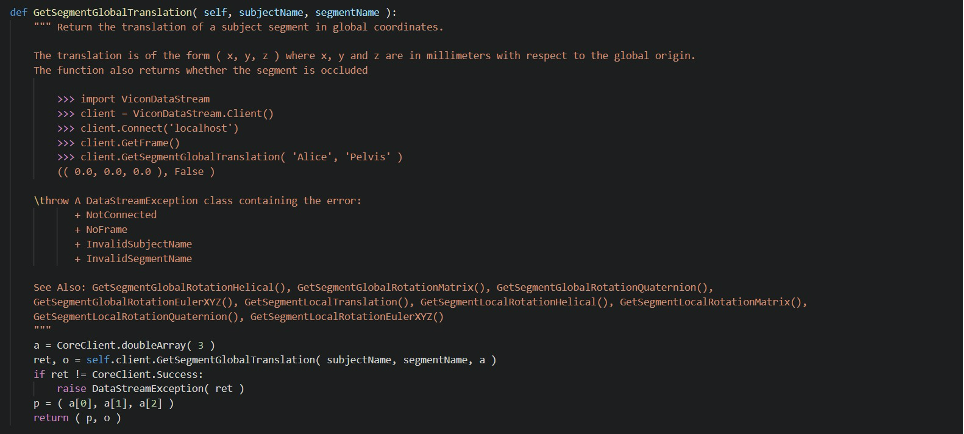
\includegraphics[width=1 \textwidth]{Relazione/Immagini/getSegmentGlobalTranslation.png}	
    \caption{Funzione utilizzata per ricevere dal Tracker il vettore posizione che rappresenta la traslazione dell'origine della terna Body di un oggetto rispetto all'origine della terna fissa Vicon, espressa nel sistema fisso Vicon}
    \label{fig:getSegmentGlobalTranslation}
\end{figure}
\\
\\
Queste funzioni restituiscono rispettivamente una struttura dati da cui poter ottenere facilmente la posizione \verb [x,y,z]  espressa in terna Vicon e la matrice di rotazione \verb (3x3)  risultante dalla composizione delle classiche rotazioni successive lungo gli assi \verb X-Y-Z  (secondo la parametrizzazione \verb "RPY" ).  
\\
\\
Il nostro scopo finale è riuscire ad inviare al Drone:

\begin{itemize}
    \item Riferimenti di posizione da inseguire utilizzando la \verb send_position_setpoint(x,y,z,0)  della classe \verb Commander .
    La posizione dovrà essere espressa nella giusta terna. Lo zero finale è il campo relativo all’angolo di Yaw "desiderato" dell’orientazione del Drone. Vedremo più avanti nel dettaglio le motivazioni alla base di questa scelta.
    \item Informazioni sulla sua posizione attuale all’interno del sistema Vicon al fine di utilizzarle per l’aggiornamento del filtro di Kalman, anche queste inviate dopo averle espresse nella terna corretta. Questo verrà fatto utilizzando la \verb send_extpos(x,y,z) .
\end{itemize}

(Nella sezione successiva riporteremo con più dettaglio tutto quanto riguarda la parte dedicata ai sistemi di riferimento e le convenzioni adottate durante l’esperimento).



\chapter*{Sistemi di Riferimento}
\addcontentsline{toc}{chapter}{Sistemi di Riferimento}
\section*{Introduzione}
\addcontentsline{toc}{section}{Introduzione}

Scendendo più nel dettaglio, qui è dove riportiamo le convenzioni che abbiamo adottato sui vari sistemi di riferimento utilizzati durante l’esecuzione degli esperimenti. 

Come mostrato in figura ~\ref{fig:SistemidiRiferimento} abbiamo deciso di adottare le seguenti terne: 
\begin{itemize} 
    \item \verb Sistema  \verb Fisso  \textbf{Vicon}  \verb (V)  : ha l’origine coincidente col centro della flight room; Gli assi \textbf{[ $X_{v}$ , $Y_{v}$ , $Z_{v}$]} sono fissi e rappresentano dunque il frame inerziale. 
    \item \verb Sistema  \verb Fisso   \textbf{Start}  ($S_{\#}$)  : ha l’origine coincidente con il \verb CDM  del \verb Drone  al momento dell’accensione. Ha dunque quota \textbf{“z”} nulla e, oltre ad essere complanare al sistema \textbf{“V”}, ha anche la sua stessa orientazione. Questo è il frame \verb navigation . 
    \item \verb Sistema  \verb Body  \textbf{Start} ($S_{i}$)  : Ha l’origine coincidente con il CDM del Drone in ogni istante \textbf{$t_{i}$}. Gli assi sono in ogni momento orientati in modo che l’asse \verb X  parta dall’origine e vada verso prua, l’asse \verb Y  parta dall’origine e vada verso sinistra (rispetto all’asse \verb X)  , l’asse \verb Z  che va dall’origine verso l’alto (\verb terna  \verb destrorsa). Rispetto ai due sistemi precedenti, la sua orientazione varia soltanto in termini di Yaw in quanto gli angoli di Pitch e Roll sono sempre supposti pari a zero. In questo modo evitiamo sia di considerare il relativo rumore nella misura di tali angoli da parte del sistema di visione, sia riusciamo a operare con sistemi di riferimento complanari (o “paralleli” nel caso prendano quota \verb z  > 0 ).
\end{itemize}
\\
Per quanto riguarda le misure fornite dal Vicon, queste sono tutte espresse in terna fissa \verb V . La parametrizzazione scelta per rappresentare posizione e orientazione del Drone all’interno del sistema \verb V   è la parametrizzazione \textbf{RPY } detta anche \textbf { XYZ }.
\\
Dato che il Drone, una volta acceso, crea il suo sistema \verb Body  in modo che abbia origine e orientazione coincidenti con quelle che assume all’istante di accensione, e dato che considera (per come abbiamo dovuto implementare il progetto) ogni riferimento in ingresso come espresso in un sistema la cui origine coincide con quela del \verb navigation  ma il cui frame è costantemente ruotato sull'asse \verb z  di un angolo pari al suo attuale angolo di \verb yaw  , abbiamo dovuto operare la conversione tra i due sistemi \textbf{V} ed {$S_{i}$} (rappresenta il sistema body del drone al generico istante \textbf{i}).
\\


\section*{Calcolo della matrice di Rotazione da \{Vicon\} a \{Body\}}
\addcontentsline{toc}{section}{Calcolo della matrice di Rotazione da \{Vicon\} a \{Body\}}
\\
Il Tracker fornisce roll ($\alpha$) pitch ($\beta$) yaw ($\gamma$) del drone rispetto al sistema di riferimento fisso Vicon \{V\}. Costruiamo dunque le varie matrici di rotazione che compongono la parametrizzazione di \textbf{Eulero XYZ} :

%
$$ R_{x} = 
\begin{bmatrix}
   1 & 0 & 0 \\
   0 & \cos(\alpha) & -\sin(\alpha)  \\
   0 & \sin(\alpha) & \cos(\alpha)
\end{bmatrix}
R_{y} = \begin{bmatrix}
   \cos(\beta) & 0 & \sin(\beta) \\
   0  & 1 & 0  \\
   -\sin(\beta) & 0 & \cos(\beta)
\end{bmatrix}
R_{z} = \begin{bmatrix}
  \cos(\gamma) & -\sin(\gamma) & 0 \\
  \sin(\gamma) & \cos(\gamma) & 0 \\
  0 & 0 & 1
\end{bmatrix}
$$
\\
In generale, introducendo soltanto per questo paragrafo una notazione più semplice, abbiamo un sistema \{V\} che costituisce il sistema inerziale e un sistema \{D\} che costituisce il sistema body del drone.
Questo sistema \{D\} solidale al drone ha il suo asse \verb X  rivolto da poppa a prua, asse \verb Y  in modo da avere una terna destrorsa con asse \verb Z  rivolto verso l'alto. 
Per riportare un vettore $P^v$ espresso in  \{V\} in un vettore $P^d$ espresso in \{D\} dobbiamo scrivere la: $P^d = R_{dv}\cdot P^v$ 
in cui la $R_{dv}$ esprime come passare "graficamente" da \{D\} a \{V\} (Per portare in realt\`a \{V\} in \{D\}). 
\\
Attraverso il prodotto delle 3 matrici otteniamo la matrice  $R_{xyz}$  che mappa un vettore in terna \{D\} in un vettore in terna \{V\}:
$$
R_{xyz} = R_{x} \cdot R_{y} \cdot R_{z} = R_{d}^v
$$
$$
R_{d}^v = \begin{bmatrix}
    \cos(\gamma)\cos(\beta) & -\cos(\beta)\sin(\gamma) & \sin(\beta) \\
    \cos(\alpha)\sin(\gamma) + \cos(\gamma)\sin(\alpha)\sin(\beta) & \cos(\alpha)\cos(\gamma) - \sin(\alpha)\sin(\beta)\sin(\gamma) & -\cos(\beta)\sin(\alpha) \\
    \sin(\alpha)\sin(\gamma) - \cos(\alpha)\cos(\gamma)\sin(\beta) & \cos(\gamma)\sin(\alpha) + \cos(\alpha)\sin(\beta)\sin(\gamma) & \cos(\alpha)\cos(\beta)
\end{bmatrix}
$$
\\
La $(R_{d}^v)$ per noi esprime come passare "graficamente" da V a D dunque ci\`o che ci serve 
\`e la sua trasposta:
$$
R_{v}^{d} = R_{zyx} = (R_{d}^v)^T
$$
$$
R_{v}^{d}=\begin{bmatrix}
    \cos(\gamma)\cos(\beta) & \cos(\alpha)\sin(\gamma) + \cos(\gamma)\sin(\alpha)\sin(\beta) & \sin(\alpha)\sin(\gamma) - \cos(\alpha)\cos(\gamma)\sin(\beta) \\
    -\cos(\beta)\sin(\gamma) & \cos(\alpha)\cos(\gamma) - \sin(\alpha)\sin(\beta)\sin(\gamma) & \cos(\gamma)\sin(\alpha) + \cos(\alpha)\sin(\beta)\sin(\gamma) \\
    \sin(\beta) & -\cos(\beta)\sin(\alpha) & \cos(\alpha)\cos(\beta)
\end{bmatrix}
$$
\\

\section*{Panoramica dei Sistemi di Riferimento}
\addcontentsline{toc}{section}{Panoramica dei Sistemi di Riferimento}

La figura ~\ref{fig:SistemidiRiferimento} rappresenta una panoramica “dall’alto” dunque la componente di traslazione lungo gli assi \verb z  non si vede ma sappiamo essere presente e necessaria in quanto il \verb Drone  per traslare dal suo punto di accensione deve aver prima preso quota; pertanto il sistema di riferimento {$S_{1}$}  avrà l’origine sicuramente ad una quota \verb z  > 0. I sistemi di riferimento {$S_{\#}$} , {$S_{\0}$}  e {$V$}  sono invece complanari a quota nulla. 

In fig.~\ref{fig:SistemidiRiferimento}  si mostra un esempio in cui il \verb drone  è inizialmente fermo all’istante $t_{0}$ (sistema di riferimento $S_{0}$ ), ha un angolo di \verb Yaw   pari a - $\psi_{0} $  ed è traslato rispetto al centro della stanza di $P_{vs}$ .
In realtà ad essere precisi {$S_{0}$}  esprime la reale posa del Drone rispetto all’osservatore nella stanza ma il Drone stesso crede di essere posizionato e orientato come espresso da {$S_{\#}$} (quindi con la stessa orientazione della terna {$V$}).
 
Successivamente all’istante $t_{1}$ il Drone risulta traslato rispetto al suo punto di accensione di $P_{sf}$ . Il che coincide con il dire che risulta essere traslato rispetto al centro della stanza di $P_{vf}$. 
Per tenere presente che negli istanti successivi a quello iniziale il Drone ha una quota \textbf{"z"  > 0} abbiamo indicato nel pedice delle traslazioni la lettera \textbf{f} come ultima in quanto rappresentativa della parola \textbf{fly}. 


\begin{figure}[h]
    \centering
    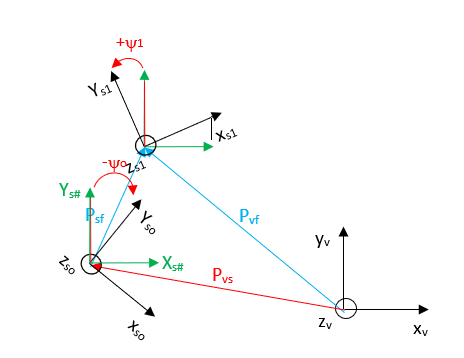
\includegraphics[width=0.8 \textwidth]{Relazione/Immagini/VICON.PNG}	
    \caption{I vari Sistemi di Riferimento introdotti}
    \label{fig:SistemidiRiferimento}
\end{figure}

Andiamo ad elencare i passaggi e le trasformazioni propri del caso rappresentato nella figura ~\ref{fig:SistemidiRiferimento}: 
\\
\begin{itemize}
    \item \textbf{Accensione del Drone in  $P_{vs}$} : il \verb Drone  crea il suo sistema di riferimento Body {$S_{0}$}  orientato come in figura.  In realtà il drone in ogni momento dell’esperimento penserà di avere angolo di \verb yaw  pari a zero in quanto noi non forniamo al filtro di Kalman le nuove misure di orientazione ma soltanto di posizione. Dunque a voler essere precisi, il Drone pensa di essere orientato esattamente come la terna {$S_{\#}$} . \\ E’ compito nostro (come vedremo di seguito) fornire riferimenti che non siano solo traslati ma anche ruotati dell’angolo di \verb Yaw  che istante per istante il drone in realtà ha rispetto a {$V$} .  
    
    \item \textbf{Creiamo dunque la matrice omogenea di rototraslazione cosi composta}:
    \\
    \\ Matrice di Rotazione da \{$S_{i}$\} a \{V\} :
    $ R_{i}^v = R_{z}(\psi_{i}) = \begin{bmatrix}
    \cos(\psi_{i}) & -\sin(\psi_{i}) & 0 \\
    \sin(\psi_{i}) & \cos(\psi_{i}) & 0 \\
    0 & 0 & 1
    \end{bmatrix}
    $
    \\
    \\
    (ricordiamo che supporremo sempre nulli gli angoli di roll e pitch)
    \\
    \\
    \\ Matrice di Rotazione da \{V\} a \{$S_{i}$\} :
    $ R_{v}^i = (R_{i}^v)^T = \begin{bmatrix}
    \cos(\psi_{i}) & \sin(\psi_{i}) & 0 \\
    -\sin(\psi_{i}) & \cos(\psi_{i}) & 0 \\
    0 & 0 & 1
    \end{bmatrix}
    $
    \\
    \\
    \\ Traslazione tra origine \{V\} e origine \{$S_{0}$\} :
    $ T_{0} = P_{vs} = \begin{bmatrix}
    x_{vs} & y_{vs} & z_{vs}
    \end{bmatrix}^T
    $
    \\
    (questa traslazione iniziale verrà continuamente convertita nella terna corrente {$S_{i}$\})
    \\
    \\
    \\ Traslazione in terna \{$S_{i}$\} :
    $ T_{si} = R_{v}^i \cdot T_{0} = \begin{bmatrix}
    \cos(\psi_{i}) & \sin(\psi_{i}) & 0 \\
    -\sin(\psi_{i}) & \cos(\psi_{i}) & 0 \\
    0 & 0 & 1
    \end{bmatrix}
    \cdot 
    \begin{bmatrix}
    x_{vs} \\ 
    y_{vs} \\
    z_{vs}
    \end{bmatrix}
    =
    \begin{bmatrix}
    x_{si} \\ 
    y_{si} \\
    z_{si}
    \end{bmatrix}
    $
    \\
    \\
    \\ Matrice Omogenea :
    $H_{si} = \begin{bmatrix}
    \cos(\psi_{i}) & \sin(\psi_{i}) & 0 & -x_{si}\\ 
    -\sin(\psi_{i}) & \cos(\psi_{i}) & 0 & -y_{si} \\
    0 & 0 & 1 & -z_{si} \\
    0 & 0 & 0 & 1
    \end{bmatrix}
    $
    \\
      \item Tralasciamo la fase di decollo in cui il \verb drone   a partire dalla sua origine iniziale prende quota lungo l’asse Z e supponiamo per semplicità di rappresentazione che non vi siano (per adesso) ulteriori rotazioni o traslazioni durante questa fase.
      \\
    \item In ogni istante il \verb Vicon  fornisce la posizione del \verb Drone  espressa nel sistema {$V$}  inizialmente pari a  $P_{vs}$  ma in generale denominata con $P_{d}^v$ che viene dunque riportata nel sistema {$S_{i}$}   prima di inviarla come misura per l’aggiornamento del filtro di Kalman. In realtà l'invio a Kalman è fatto si in ogni istante come appena detto, ma soltanto per gli istanti successivi alla fase di decollo.
    \\
    \\ Generica posizione del \verb Drone  espressa in \verb V : 
    $P_{d}^v = \begin{bmatrix}
     x_{d} & y_{d} & z_{d}   
    \end{bmatrix}^T
    $
    \\
    \\ Costruiamo il vettore omogeneo :
    $P_{dh} = \begin{bmatrix}
     x_{d} & y_{d} & z_{d} & 1 
    \end{bmatrix}^T
    $
    \\
    \\ Lo moltiplichiamo per la matrice Omogena \verb H  :
    $P_{sh} = P_{dh} \cdot H = \begin{bmatrix}
     x_{s} & y_{s} & z_{s} & 1 
    \end{bmatrix}^T
    $
    \\
    \\Lo riportiamo ad essere un vettore non omogeneo:
    $P_{d}^{si} = P_{dh} \cdot H = \begin{bmatrix}
     x_{s} & y_{s} & z_{s} 
    \end{bmatrix}^T
    $
    \\
    (Abbiamo quindi ottenuto il vettore posizione del drone non più espresso secondo la terna {$V$}  ma secondo la terna {$S_{i}$}  in quanto come detto in precedenza il drone è convinto di essere costantemente orientato come la terna {$S_{\#}$}  ed avere quindi angolo di yaw nullo. Se non avessimo proceduto alla conversione nella terna {$S_{i}$}  non sarebbe stato in grado di effettuare tale conversione in autonomia. )
    \\
    \item Supponiamo che il drone sia decollato ad esempio  ad una quota di \textbf{Z = 0.5 m} e che la Wand si trovi in posizione $P_{vf}^{v}$ (rispetto alla terna {$V$} ). Ricordiamo che l’orientazione della \verb Wand  è del tutto irrilevante ai nostri scopi e pertanto verrà sempre trascurata. A questo punto il \verb Vicon  ci fornisce $P_{vf}^{v}$ e noi la andiamo a ruotare in accordo con l'attuale orientazione della terna Body {$S_{i}$}   per poi traslarla riconducendo l'origine a quella della terna \verb navigation  . In questo modo otteniamo  come riferimento di posizione per il Drone il vettore $P_{vf}^{si}$.
    \\
    \\
    $P_{vf}^{v} = \begin{bmatrix}
       x_{vf} & y_{vf} & z_{vf}
    \end{bmatrix}^T 
    $
    , costruisco il vettore omogeneo
    $P_{vfh} = \begin{bmatrix}
       x_{vf} & y_{vf} & z_{vf} & 1
    \end{bmatrix}^T
    $
    \\
    ottengo infine : 
    $P_{vf}^{si}=H \cdot P_{vfh} = \begin{bmatrix}
       x_{sf} & y_{sf} & z_{sf} & 1
    \end{bmatrix}^T
    $
    \\
    \item A questo punto il nuovo riferimento è inviato al \verb Drone  che lo insegue. Durante il tragitto continuiamo a inviare, come prima, la sua posizione al filtro di \verb Kalman  continuando a fargli credere che il suo angolo di \verb yaw  è rimasto nullo. Possiamo farlo in quanto il riferimento che deve inseguire è già stato ruotato di conseguenza.
    \\
    \item Una volta che il \verb Drone  raggiunge la posizione desiderata, supponiamo che (a causa di eventuali disturbi durante il tragitto) abbia variato il suo angolo di \verb yaw  e che adesso sia pari a $\psi_{1}$ mostrato nella figura ~\ref{fig:SistemidiRiferimento} relativamente all’istante $t_{1}$  .  In questo caso infatti il sistema \verb Vicon  rileverà il nuovo valore dell’angolo che sarà utilizzato per ricalcolare la matrice omogenea come segue:
    \\
    \\
    \\ Matrice di Rotazione da \{$S_{1}$\} a \{V\} :
    $ R_{s1}^v = R_{z}(\psi_{1}) = \begin{bmatrix}
    \cos(\psi_{1}) & -\sin(\psi_{1}) & 0 \\
    \sin(\psi_{1}) & \cos(\psi_{1}) & 0 \\
    0 & 0 & 1
    \end{bmatrix}
    $
    \\
    \\Matrice di Rotazione da \{V\} a \{$S_{1}$\} :
    $ R_{v}^{s1} = (R_{s1}^v)^T = \begin{bmatrix}
    \cos(\psi_{1}) & \sin(\psi_{1}) & 0 \\
    -\sin(\psi_{1}) & \cos(\psi_{1}) & 0 \\
    0 & 0 & 1
    \end{bmatrix}
    $
    
    \\
    \\ Traslazione tra origine \{V\} e origine \{$S_{0}$\} :
    $ T_{0} = P_{vs} = \begin{bmatrix}
    x_{vs} & y_{vs} & z_{vs}
    \end{bmatrix}^T
    $
    \\
    \\
    \\ Traslazione ruotata in \{$S_{1}$\}  :
    $ T_{s1} = R_{v}^{s1} \cdot T_{0} = \begin{bmatrix}
    \cos(\psi_{1}) & \sin(\psi_{1}) & 0 \\
    -\sin(\psi_{1}) & \cos(\psi_{1}) & 0 \\
    0 & 0 & 1
    \end{bmatrix}
    \cdot 
    \begin{bmatrix}
    x_{vs} \\ 
    y_{vs} \\
    z_{vs}
    \end{bmatrix}
    =
    \begin{bmatrix}
    x_{s1} \\ 
    y_{s1} \\
    z_{s1}
    \end{bmatrix}
    $
    \\
    \\
    \\ Matrice Omogenea :
    $H_{s1} = \begin{bmatrix}
    \cos(\psi_{1}) & \sin(\psi_{1}) & 0 & -x_{s1}\\ 
    -\sin(\psi_{1}) & \cos(\psi_{1}) & 0 & -y_{s1} \\
    0 & 0 & 1 & -z_{s1} \\
    0 & 0 & 0 & 1
    \end{bmatrix}
    $
    \\
    \item Adesso viene ricalcolata la nuova posizione della \verb Wand  che verrà riconvertita utilizzando la nuova matrice appena calcolata per fornirla al \verb Drone  come nuovo riferimento da inseguire. Allo stesso modo continuerà ad essere inviata al filtro di Kalman la misura di posizione attuale del \verb Drone  , anch’essa fornita in sistema {$V$}  e riconvertita utilizzando la nuova matrice appena calcolata. 
    \\
    \\
    Notiamo come già ripetuto ormai più volte in precedenza che per ogni variazione all'angolo di yaw il drone continua a ricevere riferimenti di posizione da inseguire e stime della sua posizione entrambi riferiti ad un sistema posizionato sulla terna \verb navigation  ma orientata come la corrente terna \verb body  in quanto continua ad essere convinto di avere yaw nullo e pertanto noi continuiamo a inviargli informazioni in cui la "correzione" dell'orientazione è già stata calcolata.
    \\
    \item Il tutto si ripete con una frequenza di 100 Hz fin quando la \verb Wand  non viene spenta.
    \\
    \item In questo istante il sistema \verb Vicon  fornirà come posizione della Wand il valore \textbf{[0, 0, 0]}  che coincide con il valore fornito ogni qualvolta, per qualsiasi motivo, il \verb Vicon  non riesce a individuare la \verb Wand  in uno o più frame. Avendo dunque deciso di interpretare questo particolare valore di posizione come codice di errore (in quanto considerando il vincolo del pavimento e la presenza di rumore nelle misure è assolutamente improbabile se non impossibile che un oggetto si trovi in quella posizione esatta per uno o addirittura più istanti consecutivi) nel caso in cui questo venga ricevuto noi continuiamo a mantenere il drone fermo nella sua ultima posizione e, qualora il valore sia fornito per un dato numero di istanti consecutivi, decidiamo di intraprendere la fase di atterraggio per concludere quindi l’esperimento. 
    \\
\end{itemize}



\chapter*{Fasi di Test}
\addcontentsline{toc}{chapter}{Fasi di Test}

Detto quanto basta per poter comprendere il codice che siamo andati a scrivere, elenchiamo ora le varie fasi di test che abbiamo attraversato per arrivare all’esperimento finale. Le fasi sono tra loro progressive. Per alcuni test è disponibile sia il relativo file omonimo (.py), sia un video omonimo (.mp4) in cui si mostra il risultato di ciascuna esecuzione. 
\\
\\
TEST\_1.py: 
\\
In questo file abbiamo testato le funzioni della libreria py-vicon e della cf-lib che meglio riuscissero a far si che il Drone, dopo una iniziale fase di decollo, iniziasse a inseguire la posizione della Wand. In questo caso il nuovo riferimento di posizione non era dato ad ogni istante ma ad intervalli di tempo prefissati. All’interno di ogni intervallo il riferimento era mantenuto costante e pari all’ultimo inviato. Il risultato è un \textbf{“inseguimento a tratti”} della Wand da parte del Drone. 
\\
\\
Il Drone deve essere posizionato esattamente al centro della stanza e orientato esattamente come la terna fissa “V”. Soltanto dopo essersi assicurati che sia così può essere acceso e può essere eseguito l’esperimento. 
\\
\\
\\
TEST\_2.py: 
\\
A questo punto abbiamo eliminato il vincolo relativo al riferimento costante all’interno degli intervalli di tempo ed abbiamo iniziato a inviare in ogni istante (ad una frequenza di 100 Hz) la posizione corrente della Wand. Si ha dunque un “\textbf{inseguimento in tempo reale}”. 
\\
\\
\\
TEST\_3.py: 
\\
Dato che fino a questo momento l’esperimento non aveva un vero “\textbf{criterio di arresto}”, abbiamo deciso di far interrompere l’esperimento facendo atterrare gradualmente il Drone a partire dalla posizione corrente nel momento in cui la Wand viene spenta. La logica adottata è la stessa già spiegata in precedenza per cui al momento dello spegnimento della Wand si ha l’invio da parte del Vicon della particolare posizione della Wand pari a  [0, 0, 0] che abbiamo interpretato come codice di errore e che, qualora fosse fornita per diversi istanti consecutivi da logo all’inizio della procedura di atterraggio. 
\\
\\
\\
TEST\_4.py:
\\
Qui è dove abbiamo eliminato il “vincolo” di dover iniziare l’esperimento facendo partire il Drone dall’origine del sistema Vicon e con orientazione relativa rispetto alla terna “V” nulla. 
Per fare ciò abbiamo utilizzato la posizione e orientazione del Drone rispetto alla terna Vicon per creare le relative matrici omogenee di rototraslazione che permettessero di ricevere informazioni in terna Vicon e inviare riferimenti al Drone in terna Body in modo del tutto coerente secondo quanto spiegato in precedenza.
\\
\\
Il Drone può quindi essere \textbf{inizialmente posizionato ed orientato in modo del tutto arbitrario} (purchè parta ovviamente sempre dal suolo e senza pendenze).  
\\
\\

\chapter*{File Definitivo}
\addcontentsline{toc}{chapter}{File Definitivo}
\section*{Inseguimento}
\addcontentsline{toc}{section}{Inseguimento}

\\
\verb INSEGUIMENTO.py  costituisce il file definitivo ed è quello in cui abbiamo aggiunto dei flag in modo da ottenere un unico file in cui a seconda del loro valore (impostato prima dell'esecuzione e eventualmente modificato tra esecuzioni successive) otteniamo l'esecuzione di diversi rami del codice e che portano dunque all'esecuzione dell'esemperimento in diverse modalità: 
\begin{itemize}
    \item \verb MAKE_LOG_FILE: \\
    Se questo flag è posto ad 1 l'esecuzione dell'esperimento produrrà un file di log in cui saranno salvate tutte le informazioni di interesse (riferimenti inviati al drone, misure di posizione del drone inviate al filtro di Kalman, posizione e orientazione fornite da Vicon...).
     \item \verb KALMAN_INCLUDE_QUATERNION: \\
     Se questo flag è posto ad 1 l'esecuzione prevederà che il drone riceva dal sistema Vicon oltre che all'informazione di posizione anche quella di orientamento (fornita per mezzo di quaternioni).
     \item \verb ACTIVATE_KALMAN_DURING_TAKEOFF: \\
     Se questo flag è posto ad 1 l'esperimento avrà luogo in modo che anche durante il decollo il drone riceva informazioni per l'aggiornamento del filtro di Kalman (posizione o posa a seconda del valore del precedente flag). 
     \item \verb LOG_TEST_WITH_DISACTIVATED_THRUSTER: \\
     Questo falg se abilitato consente di condirre esperimenti a mano libera, senza bisogno della wand e a "motori spenti" in modo da poter muovere il drone nello spazio semplicemente prendendolo in mano e guidandolo dove vogliamo. Durante questo tipo di esecuzione le informazioni raccolte dipenderanno dai valori assegnati ai flag precedenti. 
\end{itemize}
\\
\\
Facciamo presente che tutta la parte di relazione finora descritta è riferita al caso in cui i valori dei flag sono rispettivamente: 
\begin{itemize}
    \item \verb MAKE_LOG_FILE: 1 
    \item \verb KALMAN_INCLUDE_QUATERNION: 0
    \item \verb ACTIVATE_KALMAN_DURING_TAKEOFF: 0
    \item \verb LOG_TEST_WITH_DISACTIVATED_THRUSTER: 0
\end{itemize}
\\
Facciamo presente che dal codice si nota una prima sezione in cui oltre ai flag appena spiegati è possibile modificare quelle variabili che, a seconda di dove l'esperimento è condotto o di chi lo sta conducendo, potrebbero assumere valori diversi e che pertanto abbiamo reso "parametrici" in modo che possano essere semplicemente modificate una sola volta prima dell'esecuzione senza rendere necessarie modifiche interne al codice vero e proprio. A titolo di esempio, stiamo parlando di variabili come "nome associato agli oggetti nel sistema Vicon", "URL della connessione tra Crazyradio e Crazyflie", "IP e porta di connessione relative al sistema Vicon"...
\\
\section*{Relativo}
\addcontentsline{toc}{section}{Relativo}
\\
In aggiunta al file \verb INSEGUIMENTO.py  abbiamo fornito un file analogo ma denominato \verb RELATIVO.py  e per cui vale tutto quanto detto finora ad eccezione del fatto che l'esecuzione non prevede l'inseguimento del moto della Wand ma il Drone, una volta decollato, a partire dalla sua posizione corrente insegue soltanto il moto relativo della Wand. Ad esempio, se la Wand “disegnerà” nello spazio un quadrato a partire dalla sua posizione iniziale, il Drone, a partire anch’esso dalla sua posizione iniziale (diversa ovviamente da quella della Wand) replicherà nello spazio il “disegno” del quadrato fatto dalla Wand. Il tutto in tempo reale ad una frequenza di 100 Hz.
\\
La trattazione di quest’ultima modalità non è riportata in quanto si basa esattamente sugli stessi concetti spiegati finora e validi per la prima modalità; l’unica differenza è costituita appunto dal riferimento di posizione inviato al drone che non è più coincidente con la nuova posizione della Wand ma diventa coincidente alla posizione attuale del Drone a cui viene sommata la \textbf{traslazione} che la Wand ha compiuto rispetto alla sua ultima posizione.
\\
\\
\section*{Interfaccia}
\addcontentsline{toc}{section}{Interfaccia}
\\
Come ulteriore possibile sviluppo forniamo un file \verb INTERFACCIA.py  in cui abbiamo implentato una prima semplicissima interfaccia da cui rendiamo possibile consultare un file README.txt (riportato nell'ultima sezione di questa relazione) in cui sono contenute le istruzioni su come poter essere in grado (come noi) a partire da zero di poter eseguire l’esperimento. Qui troviamo le indicazioni su come si deve predisporre l’ambiente, quali librerie dover installare, quali sono le osservazioni più importanti e la procedura da dover seguire per la corretta riuscita dell’esperimento. Da questa semplice interfaccia è inoltre possibile cliccare su un pulsante \verb START  ed eseguire quindi uno soltanto dei due file sopra descritti (\verb INSEGUIMENTO  , \verb RELATIVO  ). Precisiamo che, se eseguito così come è scritto, il file \verb INTERFACCIA.py  eseguirà soltanto un banale esempio di prova in cui viene calcolato randomicamente un numero intero per poi stamparlo nel form dopo un ciclo di attesa di molte iterazioni (questo per testare il fatto che click consecutivi successivi al primo sul pulsante start sono disabilitati dirante l'esecuzione del codice lanciato) . 
\\
Qualora si voglia utilizzare il file per eseguire l'esperimento vero e proprio si prega di leggere attentamente i vari commenti presenti tra le righe di codice e di seguire la procedura riportata nel file README.txt. 


\section*{Possibili Sviluppi}
\addcontentsline{toc}{section}{Possibili Sviluppi}
\\
Volendo pensare a possibili sviluppi futuri, le nostre idee sono state le seguenti: 
\begin{itemize}
    \item Sicuramente come prima cosa dovrebbe essere trovato un modo per poter inviare al Drone anche le misure di orientazione senza inficiare sulle performance del volo. Attualmente infatti volendo inviare al filtro di Kalman del Drone anche l'informazione dell'orientazione contenuta nei quaternioni (per poter quindi evitare di "pre-ruotare" le informazioni inviate e lasciare che il Drone stesso effettui questa correzione) otteniamo come risultato una instabilità durante il volo che ne causa la caduta immediata. 
    \\
    Tra gli elementi emersi durante l'analisi di questo problema e classificati come "possibili cause" facciamo presente che, come si può evincere plottando i file di log (presenti nella cartella /LOG) i valori dell'angolo di Pitch forniti dal Vicon e ottenuti dalla tabella di log del Drone risultano essere di segno opposto; inoltre, sempre dal confronto tra i valori forniti dal Vicon e quelli ottenuti dalla tabella di log del Drone, emergono vari ritardi più o meno marcati a seconda delle condizioni in cui si effettuano gli esperimenti. 
    \item In secondo luogo si può pensare di estendere l'interfaccia in modo che contenga più pulsanti al fine di poter lanciare indifferentemente una tra le due versioni disponibili (inseguimento del moto assoluto e relativo) senza bisogno di attuare ogni volta la procedura di modifica dei nomi dei relativi file e dei relativi codici. 
    \item Una volta implementati i punti precedenti si può pensare di replicare quanto appreso da questo esperimento per riprodurne uno che utilizzi non un solo drone ma una formazione. 
\end{itemize}








\verbatiminput{Relazione/Capitoli/README.txt}

\end{document}